\chapter{Estado de la cuestión}
\label{cap:estadoDeLaCuestion}

---Introduccion breve---

\section{Herramientas de edición de mallas existentes}

En esta sección se explica brevemente la historia y algunas de las alternativas de editores de mallas existentes, y el motivo del desarrollo del programa frente al uso de estas.

\subsection{Historia}

El origen de la edición interactiva de gráficos por computador se remonta a Sketchpad, desarrollado por Ivan Sutherland en 1963, un programa que permitió cambiar la comunicación con los ordenadores de instrucciones escritas, a poder interactuar mediante dibujos y manipulaciones de objetos directamente sobre una pantalla~\cite{sketchpad0,sketchpad,sketchpad_history}.

Las primeras herramientas comerciales de modelado 3D surgieron en la década de 1980. Wavefront Technologies, fundada en 1984 por Bill Kovacs, Larry Barels y Mark Sylvester desarrolló \emph{The Advanced Visualizer}, un conjunto de programas para la creación de gráficos por computador, para el cual definió el formato OBJ (sección~\ref{sec:obj}). De forma paralela, Alias Research, que pasaría posteriormente a denominarse Alias Systems Corporation antes de ser adquirida por Autodesk en 2006, desarrolló PowerAnimator, una herramienta de modelado y animación usada ampliamente en la industria del cine. En 1995, ambas compañías fueron adquiridas por Silicon Graphics y fusionadas en Alias|Wavefront, cuya tecnología combinada dio lugar en 1998 al lanzamiento de Maya \cite{maya_history}.

De forma independiente, Ton Roosendaal escribió en enero de 1994 el código fuente de lo que llegaría a ser Blender, inicialmente como herramienta interna del estudio de animación NeoGeo. En octubre de 2002, tras el cierre de la compañía que lo comercializaba (Not a Number), se publicó como software libre mediante una campaña de recaudación que permitió comprar los derechos sobre su código fuente, y procedería a convertirse en una de las herramientas de edición de mallas más reconocidas a día de hoy\cite{blender_history}.

\subsection{Blender}

Blender es un conjunto de herramientas de creación 3D de código abierto que cubre modelado, esculpido, animación, simulación, renderizado y composición dentro de una única aplicación \cite{blender}. Su modo de edición de mallas (\emph{Edit Mode}) trabaja con los mismos tres tipos de elementos seleccionables que este proyecto (vértices, aristas y caras), y ofrece un control explícito sobre el comportamiento de operaciones como la eliminación de elementos, permitiendo al usuario decidir cuánta geometría conectada desea conservar (sección~\ref{sec:eliminacion}).

\subsection{Autodesk Maya}

Maya es una herramienta de modelado y animación 3D de uso extendido en la industria del cine y los videojuegos, heredera directa de la tecnología de Alias|Wavefront. A diferencia de Blender, su modelo de licencia es comercial, y su conjunto de herramientas de edición de mallas está pensado para integrarse dentro de \emph{pipelines} de producción más amplios \cite{maya}.

\subsection{Motivación de desarrollo frente a otras opciones}

Frente a Blender y Maya, herramientas de propósito general con décadas de desarrollo detrás, el editor desarrollado en este trabajo se plantea como una herramienta de propósito acotado, centrada específicamente en las operaciones fundamentales de edición de mallas poligonales: selección, transformación, eliminación y extrusión. Esto permite dedicar el trabajo a comprender e implementar en profundidad los fundamentos de estas operaciones.

\section{Tecnologías utilizadas}

A continuación se describen brevemente las distintas tecnologías utilizadas en el transcurso del proyecto y el motivo de su uso.

\subsection{OpenGL}

Para desarrollar una aplicación gráfica, el proyecto requiere una API gráfica que permita renderizar modelos tridimensionales, gestionar \textit{shaders} y mantener la posibilidad de ejecutar la aplicación en distintos sistemas operativos.

OpenGL (\emph{Open Graphics Library}) es una especificación abierta y multiplataforma para el desarrollo de aplicaciones que produzcan gráficos 2D y 3D. Fue desarrollada originalmente por Silicon Graphics Inc. y publicada por primera vez en 1992. Desde 2006, su desarrollo y mantenimiento corren a cargo de Khronos Group, un consorcio industrial fundado en el año 2000, que ha continuado publicando nuevas versiones de la especificación hasta la actualidad \cite{opengl, openGL_history}.

Para el proyecto se consideran varias alternativas comunes para aplicaciones gráficas: Direct3D, Vulkan y OpenGL. Direct3D es una API gráfica propietaria desarrollada por Microsoft, disponible únicamente en Windows. Vulkan, gestionada también por Khronos Group, es una API de bajo nivel que ofrece un control explícito sobre los recursos de la GPU (gestión de memoria, sincronización de comandos, etc.), a cambio de una mayor complejidad en el código. OpenGL, en cambio, ofrece un nivel de abstracción más alto, delegando en el controlador gráfico buena parte de la gestión de recursos, y cuenta con una documentación extensa y numerosas bibliotecas de utilidad desarrolladas por la comunidad.

La primera consideración para escoger el candidato adecuado fueron las capacidades multiplataforma de la API. Debido a que Direct3D únicamente ofrece soporte para Windows, queda descartada como opción. Entre OpenGL y Vulkan, se opta por OpenGL: su curva de aprendizaje más reducida, su documentación extensa y el acceso a numerosas bibliotecas de utilidad la convierten en la opción más apropiada para el proyecto. A esto se suma la familiaridad previa con OpenGL, adquirida durante el grado, lo que facilita su uso durante el desarrollo del proyecto.

\subsection{glad}

En la mayoría de plataformas, el sistema operativo solo expone de forma directa (estática) las funciones correspondientes a OpenGL 1.1. El acceso a las funciones introducidas en versiones posteriores, así como a las extensiones específicas del controlador gráfico, requiere obtener el puntero a cada función en tiempo de ejecución, una vez creado el contexto de OpenGL, mediante mecanismos propios de cada plataforma (por ejemplo, \texttt{wglGetProcAddress} en Windows o \texttt{glXGetProcAddress} en Linux) \cite{opengl-loading}. Realizar este proceso manualmente para cada función resulta tedioso y propenso a errores, además de obligar a escribir código distinto para cada sistema operativo, lo cual compromete la portabilidad buscada en el proyecto.

Para evitar este trabajo repetitivo, se usa glad, una biblioteca que genera automáticamente, a partir de las especificaciones oficiales de Khronos Group, el código necesario para cargar en tiempo de ejecución los punteros a las funciones compatibles con la versión de OpenGL utilizada, abstrayendo además las diferencias entre plataformas.

\subsection{glm}

Un requisito de un editor de mallas es poseer la capacidad de realizar operaciones matriciales, alternar entre los distintos sistemas de coordenadas empleados en la representación tridimensional (modelo, vista y proyección), y transformar coordenadas de pantalla a coordenadas del mundo (por ejemplo, para implementar la selección de elementos mediante \emph{ray casting}), entre otras. Con este fin, glm es una biblioteca que se adapta a las necesidades de este trabajo, ofreciendo las operaciones matemáticas de vectores y matrices en las que se apoyan este tipo de funcionalidades en aplicaciones gráficas \cite{glm}.

\subsection{Qt}

Qt es un framework multiplataforma para el desarrollo de interfaces gráficas, originado en 1991 de la mano de Haavard Nord y Eirik Chambe-Eng, cuya primera versión pública se publicó en 1995 bajo la empresa Trolltech. Desde entonces, su desarrollo ha continuado bajo distintas compañías, siendo en la actualidad mantenido por The Qt Company junto con la comunidad de código abierto del Qt Project. Qt posee capacidad de creación de ventanas y elementos de interfaz de usuario \cite{qt, qt-history}.

El proyecto requiere una ventana de renderizado, además de gestión del contexto de OpenGL y del input del usuario. Para la creación del contexto de OpenGL y de la ventana se consideró GLFW, una biblioteca multiplataforma que ofrece una API sencilla centrada exclusivamente en estos fines, y que constituye una alternativa habitual a frameworks más completos como Qt cuando no se necesita un sistema de interfaz de usuario elaborado. Qt, por su parte, además de estas capacidades básicas, incorpora un extenso conjunto de widgets y herramientas para la construcción de interfaces gráficas complejas (menús, paneles, diálogos, etc.).

Dado que el proyecto, más allá de la ventana de renderizado, requiere una interfaz de usuario con distintos paneles y controles para la edición de mallas, las herramientas de creación de elementos de interfaz que ofrece Qt fueron el motivo de su elección frente a GLFW.

\subsection{Mallas}
Una malla poligonal es la estructura de datos habitual para representar la superficie de un objeto tridimensional. Está formada por un conjunto de vértices, cada uno de los cuales almacena, como mínimo, una posición en el espacio, y opcionalmente otros atributos como su normal o sus coordenadas de textura. Los vértices se conectan mediante aristas, y los conjuntos de aristas que forman un contorno cerrado delimitan una cara, la unidad básica que compone la superficie del objeto.

Aunque una cara puede estar formada, en principio, por cualquier número de vértices, en gráficos por computador en tiempo real las mallas se representan casi siempre mediante caras triangulares: al ser un polígono siempre plano y convexo, un triángulo no presenta ambigüedades a la hora de ser rasterizado, lo que simplifica su procesamiento por parte de la GPU. Aquellas mallas que originalmente contienen caras con más de tres vértices (por ejemplo, cuadriláteros) se descomponen en triángulos mediante un proceso de triangulación antes de ser renderizadas.

En cuanto a su representación en memoria, una malla se almacena habitualmente como una lista de vértices junto con una lista de caras, donde cada cara no repite la información de sus vértices, sino que hace referencia a ellos mediante sus índices dentro de la lista de vértices, dando lugar a lo que se conoce como malla indexada (sección \ref{sec:almacenamiento-mallas}).

\subsection{Almacenamiento de mallas} \label{sec:almacenamiento-mallas}

Existen numerosos formatos de archivo para el almacenamiento de mallas tridimensionales, cada uno orientado a distintos casos de uso: formatos como FBX o glTF permiten representar escenas completas, con jerarquías de objetos, animaciones y materiales complejos, mientras que otros, como OBJ (\emph{Wavefront Object}), se centran en representar de forma sencilla la geometría de una malla individual (vértices, normales, coordenadas de textura y caras), junto con sus materiales básicos en un archivo asociado (MTL). Por su simplicidad y su amplia adopción como formato de intercambio, OBJ es habitual como formato de entrada en herramientas de edición de mallas centradas en la geometría, sin necesidad de gestionar información adicional de escena o animación.

Para importar estos archivos a la herramienta de edición se necesita una biblioteca de carga. Una opción popular es Assimp, que permite importar archivos en numerosos formatos, frente al formato único que soporta tinyobjloader (OBJ).

Tinyobjloader ofrece tanto una integración más sencilla como una menor complejidad de uso, por lo que resulta la mejor opción para el proyecto, junto con el formato OBJ.

\section{Conceptos y técnicas de gráficos 3D}

\subsection{Pipeline gráfico} \label{sec:pipeline-grafico}

El \textit{pipeline} gráfico (\emph{graphics pipeline}) es la secuencia de etapas mediante la cual una GPU transforma los datos de una escena tridimensional en una imagen bidimensional. Aunque su implementación concreta varía entre APIs, sus etapas principales son las siguientes.

En primer lugar, el \emph{vertex shader} procesa cada vértice de la malla de forma individual, aplicando sobre él las transformaciones necesarias para llevarlo desde su sistema de coordenadas local hasta el espacio de recorte (sección \ref{sec:pipeline-coordenadas}). A continuación, la etapa de ensamblado de primitivas (\emph{primitive assembly}) agrupa los vértices procesados en primitivas geométricas (triángulos), y realiza el recorte (\emph{clipping}) de aquellas que quedan parcial o totalmente fuera del volumen visible, así como, opcionalmente, el descarte de caras no orientadas hacia la cámara (\emph{culling}).

Estas primitivas pasan después por la etapa de rasterización, que las convierte en un conjunto de fragmentos: unidades discretas asociadas a las posiciones de píxel que la primitiva cubre en pantalla, e interpolando entre los vértices los datos asociados a cada una (color, normales, coordenadas de textura, etc.). Cada fragmento es procesado individualmente por el \emph{fragment shader}, encargado de calcular su color final, típicamente a partir de cálculos de iluminación y texturizado. Por último, los fragmentos resultantes son sometidos a una serie de operaciones por fragmento (test de profundidad, de \emph{stencil}, mezcla de color, entre otras) que determinan si son escritos en el \emph{framebuffer} y cómo se combinan con el contenido ya existente en él, dando lugar a la imagen final.

Tanto el \emph{vertex shader} como el \emph{fragment shader} están escritas en un lenguaje de \emph{shading}, como GLSL en el caso de OpenGL, lo que permite personalizar el comportamiento del \textit{pipeline} para cada aplicación.

\subsection{Pipeline de coordenadas} \label{sec:pipeline-coordenadas}

Para representar en una pantalla bidimensional un elemento que existe en un espacio tridimensional, es necesario aplicar sobre él una secuencia de transformaciones, cada una de las cuales lo lleva de un sistema de coordenadas al siguiente. Estas transformaciones son las que se aplican durante la etapa de \emph{vertex shader} del \textit{pipeline} gráfico (sección \ref{sec:pipeline-grafico}).

Un objeto se describe en unas coordenadas locales, definidas respecto al origen que tenía en el momento de su creación. Multiplicando la posición de cada vértice por una matriz de modelado, se obtienen sus coordenadas globales o de mundo: el espacio compartido en el que coexisten una o más mallas, cada una posicionada respecto a un mismo origen común.

A continuación, se aplica una matriz de vista, que transforma dichas coordenadas de mundo a coordenadas relativas a una cámara: una abstracción definida por una posición y una orientación, que determina desde dónde y hacia dónde se observa la escena. Es en este paso donde se obtiene una representación de cómo se observarían los objetos del mundo desde la perspectiva de dicha cámara. La cámara, como cualquier otro elemento de la escena, puede trasladarse y rotar libremente dentro del mundo; sin embargo, en su propio sistema de referencia permanece siempre situada en el origen y orientada en una dirección fija, siendo el resto del mundo el que se transforma en relación a ella al aplicar la matriz de vista.

A continuación, se aplica una matriz de proyección, que transforma dichas coordenadas de cámara al espacio de recorte (\emph{clip space}). Esta matriz determina el volumen de la escena que resulta visible, descartando aquello que quede fuera de él y difiere según el tipo de proyección empleada, en perspectiva u ortogonal, y lo proyecta sobre un plano.

Las coordenadas de recorte no son directamente utilizables: es necesario dividir sus tres primeras componentes entre su cuarta componente, un paso conocido como división de perspectiva, para obtener las coordenadas normalizadas de dispositivo (\emph{normalized device coordinates}, NDC), en las que la escena visible queda representada dentro de un cubo de lado 2 centrado en el origen (las coordenadas van desde -1 a 1). Finalmente, mediante la transformación de \emph{viewport}, estas coordenadas normalizadas se convierten en coordenadas de pantalla (\emph{screen space}), expresadas en píxeles y referidas a las dimensiones reales de la ventana de renderizado (figura \ref{fig:transformacion-coordenadas}).

\begin{figure}[htbp]
    \centering
    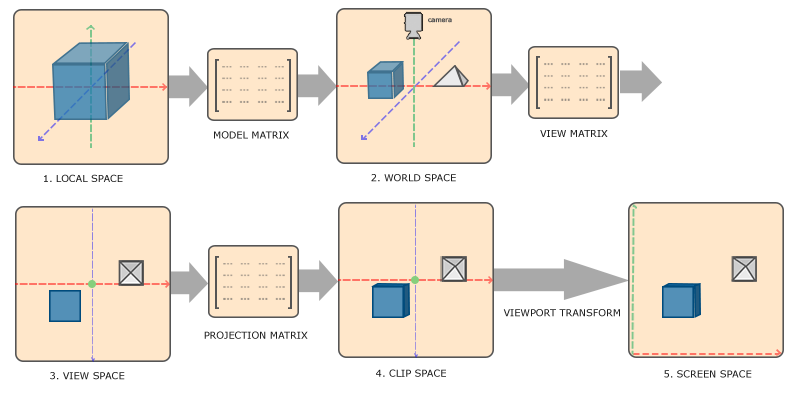
\includegraphics[width = 1\textwidth]{TFGTeXiS-UTF8/Imagenes/Bitmap/coordinate_systems.png}
    \caption{Pipeline de transformación de coordenadas.}\cite{learnOpenGL_coordinateSystems}
    \label{fig:transformacion-coordenadas}
\end{figure}

\subsection{Buffers de geometría en OpenGL}

En el \emph{core profile} de OpenGL utilizado en aplicaciones modernas no es posible renderizar geometría directamente desde estructuras de datos en memoria de la CPU: es necesario almacenar previamente dicha información en memoria de la GPU, mediante objetos específicos para este fin. Esto supone un cambio respecto al llamado modo inmediato (\emph{immediate mode}), disponible en versiones antiguas de OpenGL y en el \emph{compatibility profile}, en el que los vértices podían especificarse y transmitirse a la GPU en cada frame. Dicho enfoque quedó obsoleto por su impacto negativo en el rendimiento, especialmente en el caso de geometría estática. 

Para transmitir y organizar la geometría de una malla se emplean habitualmente tres tipos de objetos:

\begin{itemize}
    \item \emph{Vertex Buffer Object} (VBO): almacena los atributos de los vértices (posición, normal, coordenadas de textura, entre otros) que serán utilizados durante el renderizado. Al cargar esta información una única vez en memoria de GPU, se evitan transferencias repetidas entre CPU y GPU en cada frame.
    \item \emph{Element Buffer Object} (EBO), también conocido como \emph{index buffer}: almacena una lista de índices que hacen referencia a los vértices del VBO, en lugar de repetir sus atributos por cada triángulo que los utiliza. Esta técnica de renderizado, en la que la geometría se referencia mediante índices en vez de duplicar vértices, se conoce como \textbf{malla indexada}.
    \item \emph{Vertex Array Object} (VAO): almacena la configuración necesaria para que la GPU sea capaz de interpretar los atributos contenidos en el VBO: cuántos atributos hay, de qué tipo son, y en qué posición de memoria se encuentra cada uno dentro de la estructura de cada vértice.
\end{itemize}

El conjunto formado por un VAO junto con el VBO (y, en su caso, el EBO) que referencia constituye la representación en GPU de una malla, a la que se hace referencia mediante el identificador de dicho VAO en las llamadas de renderizado.

\subsection{Selección de elementos en aplicaciones 3D}

En aplicaciones interactivas de edición 3D es habitual que el usuario deba señalar con el ratón un elemento concreto de una escena tridimensional, un proceso conocido como \emph{picking}. Existen distintas técnicas para resolver este problema, que difieren en el espacio en que se realiza la comparación y en su coste computacional.

El \emph{raycasting} consiste en proyectar un rayo desde la posición del ratón hacia la escena, y determinar con qué elementos de la geometría dicho rayo intersecta \ref{raycasting}. Una alternativa consiste en proyectar la geometría tridimensional al espacio de pantalla y comparar directamente en dos dimensiones frente a la posición del ratón, evitando el cálculo de intersecciones del rayo y la geometría en tres dimensiones.

Una tercera técnica, conocida como \emph{back-buffer selection} o selección mediante búfer auxiliar, evita por completo el cálculo geométrico de proximidad: la escena se renderiza en un búfer fuera de pantalla, asignando a cada elemento seleccionable un color plano único que codifica su identificador, y la selección se resuelve leyendo el color del píxel bajo el cursor y decodificándolo de vuelta a dicho identificador \cite{3dkingdoms-selection}. Esta técnica ofrece una selección exacta a nivel de píxel sin necesidad de ningún cálculo de distancia o intersección, a cambio de requerir una pasada de renderizado adicional y una lectura síncrona del contenido de la GPU hacia la CPU (\texttt{glReadPixels}), una operación que puede introducir una espera hasta que la GPU termine de procesar dicha pasada.

\subsection{Raycasting} \label{raycasting}

El \emph{raycasting} es una técnica que consiste en proyectar un rayo y determinar con qué elementos de la geometría de una escena intersecta.

En el caso de mallas poligonales, dado que estas se componen de caras triangulares, la intersección del rayo con la malla se reduce a comprobar su intersección individual con cada uno de sus triángulos, un problema conocido como intersección rayo-triángulo. Existen distintos algoritmos para resolverlo. Uno de los más empleados es el algoritmo de Möller–Trumbore, que calcula el punto de intersección, si existe, en términos de sus coordenadas baricéntricas respecto al triángulo, sin necesidad de precalcular la ecuación del plano que lo contiene.

El raycasting tiene aplicación en múltiples ámbitos de los gráficos por computador, como la detección de colisiones o la selección de elementos de una escena mediante el ratón, proyectando un rayo desde la posición del cursor hacia el interior de la escena y determinando el primer elemento con el que intersecta.
